\documentclass[twocolumn,10pt,journal]{IEEEtran}
\usepackage{subfigure}
\usepackage{graphicx}

\title{Demonstration of ``matlab-figure-formatter''}
\author{Junwei He\thanks{%
  e-mail: hejw56@mail2.sysu.edu.cn.
}}

\begin{document}

\maketitle

\begin{figure}
  \centering
  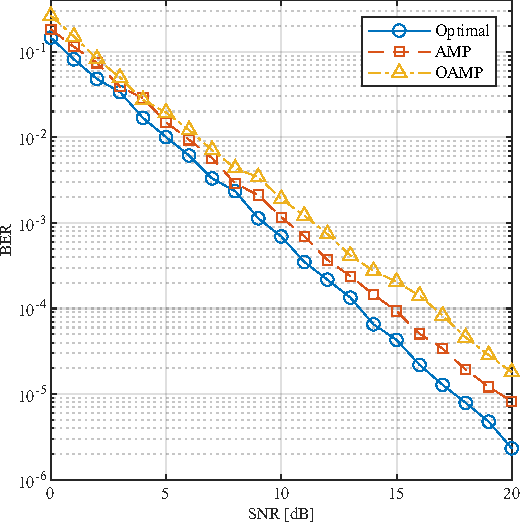
\includegraphics{figure/example_single_4x4.pdf}
  \caption{Single-column, single-panel figure with an overall aspect ratio of 4:4. MATLAB command: \texttt{formatFigure(100, 1)}.}
\end{figure}

\begin{figure}
  \centering
  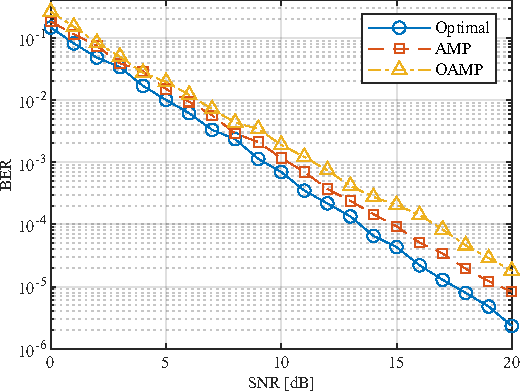
\includegraphics{figure/example_single_4x3.pdf}
  \caption{Single-column, single-panel figure with an overall aspect ratio of 4:3. MATLAB command: \texttt{formatFigure(100, 0.75)}.}
\end{figure}

\begin{figure}
  \centering
  \subfigure[]{%
    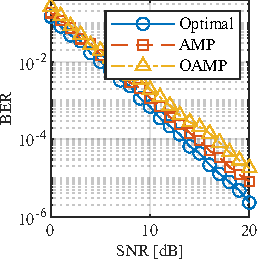
\includegraphics{figure/example_horizontal2_4x2.pdf}%
  }%
  \subfigure[]{%
    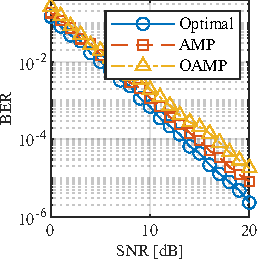
\includegraphics{figure/example_horizontal2_4x2.pdf}%
  }
  \caption{Single-column figure with two horizontally arranged panels and an overall aspect ratio of 4:2. MATLAB command: \texttt{formatFigure(50, 1)}.}
\end{figure}

\begin{figure}
  \centering
  \subfigure[]{%
    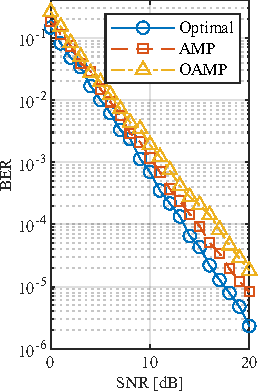
\includegraphics{figure/example_horizontal2_4x3.pdf}%
  }%
  \subfigure[]{%
    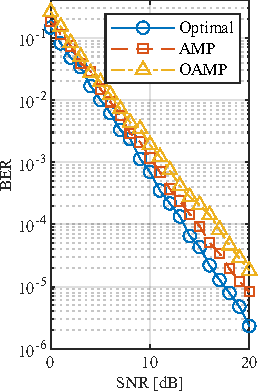
\includegraphics{figure/example_horizontal2_4x3.pdf}%
  }
  \caption{Single-column figure with two horizontally arranged panels and an overall aspect ratio of 4:3. MATLAB command: \texttt{formatFigure(50, 1.5)}.}
\end{figure}

\begin{figure}
  \centering
  \subfigure[]{%
    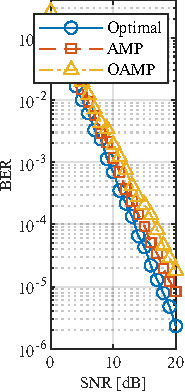
\includegraphics{figure/example_horizontal3_4x3.pdf}%
  }%
  \subfigure[]{%
    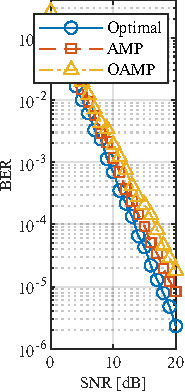
\includegraphics{figure/example_horizontal3_4x3.pdf}%
  }%
  \subfigure[]{%
    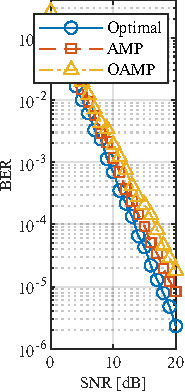
\includegraphics{figure/example_horizontal3_4x3.pdf}%
  }
  \caption{Single-column figure with three horizontally arranged panels and an overall aspect ratio of 4:3. MATLAB command: \texttt{formatFigure(100/3, 9/4)}.}
\end{figure}

\begin{figure}
  \centering
  \subfigure[]{%
    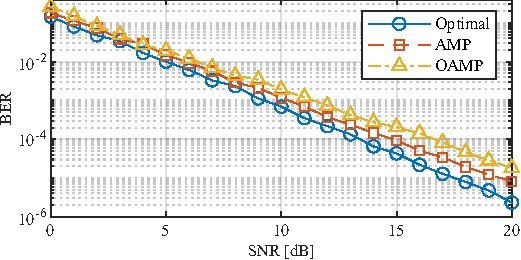
\includegraphics{figure/example_vertical2_4x4.pdf}%
  }

  \subfigure[]{%
    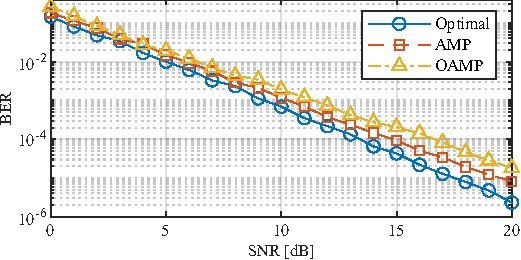
\includegraphics{figure/example_vertical2_4x4.pdf}%
  }
  \caption{Single-column figure with two vertically arranged panels and an overall aspect ratio of 4:4. MATLAB command: \texttt{formatFigure(100, 0.5)}.}
\end{figure}

\begin{figure}
  \centering
  \subfigure[]{%
    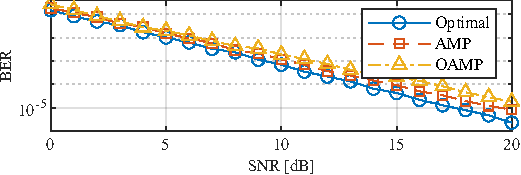
\includegraphics{figure/example_vertical3_4x4.pdf}%
  }

  \subfigure[]{%
    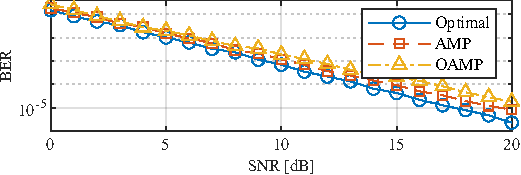
\includegraphics{figure/example_vertical3_4x4.pdf}%
  }

  \subfigure[]{%
    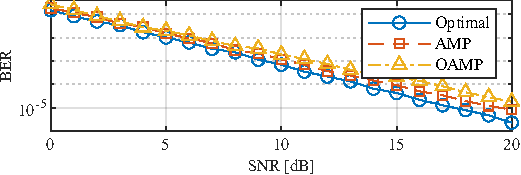
\includegraphics{figure/example_vertical3_4x4.pdf}%
  }
  \caption{Single-column figure with three vertically arranged panels and an overall aspect ratio of 4:4. MATLAB command: \texttt{formatFigure(100, 1/3)}.}
\end{figure}

\begin{figure*}
  \centering
  \subfigure[]{%
    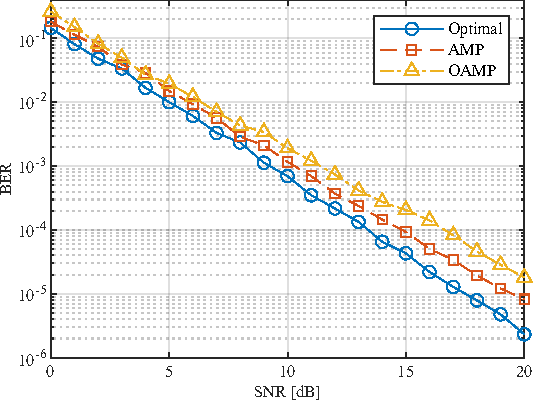
\includegraphics{figure/example_horizontal2_8x3_double.pdf}%
  }%
  \subfigure[]{%
    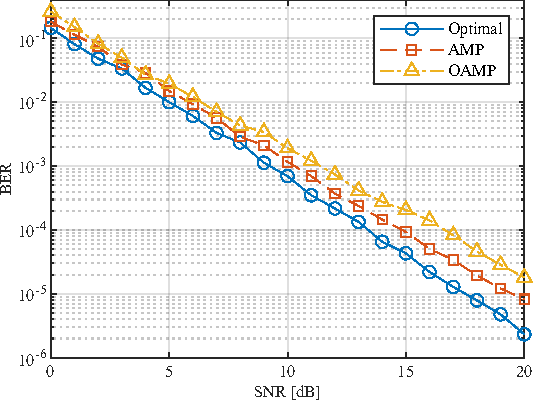
\includegraphics{figure/example_horizontal2_8x3_double.pdf}%
  }
  \caption{Double-column figure with two horizontally arranged panels and an overall aspect ratio of 8:3. MATLAB command: \texttt{formatFigure(100/2, 3/4, "double")}.}
\end{figure*}

\begin{figure*}
  \centering
  \subfigure[]{%
    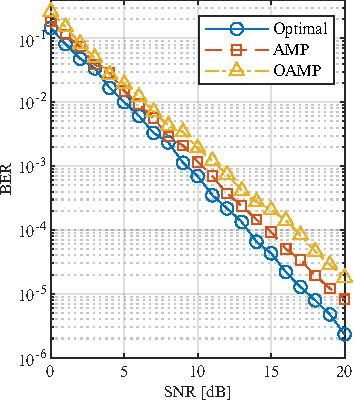
\includegraphics{figure/example_horizontal3_8x3_double.pdf}%
  }%
  \subfigure[]{%
    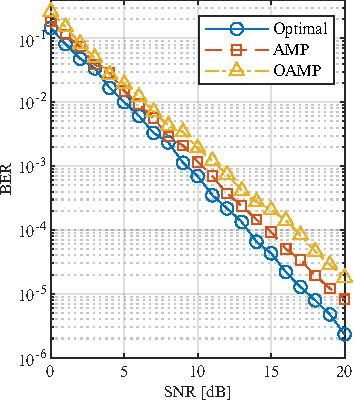
\includegraphics{figure/example_horizontal3_8x3_double.pdf}%
  }%
  \subfigure[]{%
    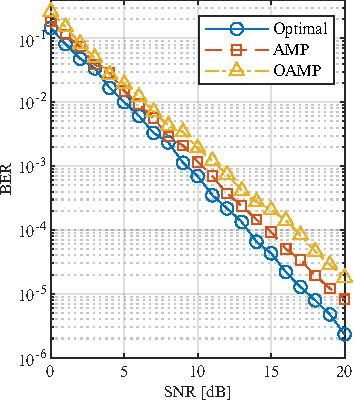
\includegraphics{figure/example_horizontal3_8x3_double.pdf}%
  }
  \caption{Double-column figure with three horizontally arranged panels and an overall aspect ratio of 8:3. MATLAB command: \texttt{formatFigure(100/3, 9/8, "double")}.}
\end{figure*}

\begin{figure}
  \centering
  \subfigure[]{%
    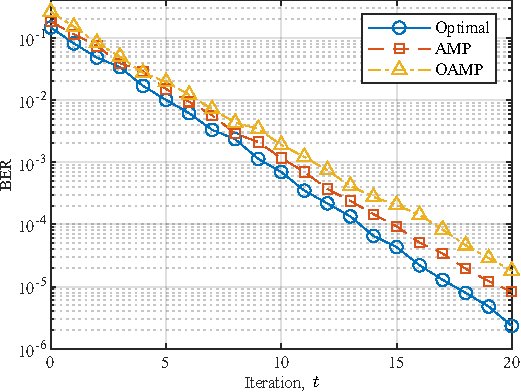
\includegraphics{figure/example_single_4x3_xlabel.pdf}%
  }%
  
  \subfigure[]{%
    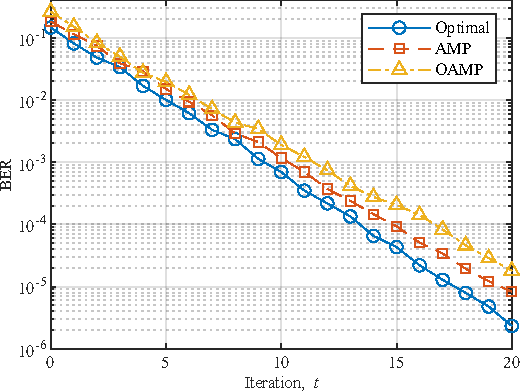
\includegraphics{figure/example_single_4x3_xlabel_0.pdf}%
  }%
  
  \caption{Comparison of axis labels with and without LaTeX-formatted mathematical symbols. Precise alignment requires additional adjustments and is generally unnecessary for routine plotting. MATLAB function: \texttt{xlabel\_Iteration\_formatter}.}
\end{figure}

\end{document}